%!TEX root = ../main.tex
\section{Περιγραφή \& Ανάλυση Προβλήματος}

Στην παρούσα διπλωματική εργασία, ο τελικός στόχος είναι η υλοποίηση ενός ενσωματωμένου συστήματος για την αναγνώριση ακμών με τη μέθοδο του Canny. Αρχικά, θα αξιολογηθεί η σύνθεση της βασισμένης σε C++ υλοποίησης και στη συνέχεια θα υλοποιηθεί ένα πλήρες σύστημα για τη μεταφορά δεδομένων ανάμεσα στην προγραμματιζόμενη λογική και τον ενσωματωμένο επεξεργαστή. Για την επίτευξη του στόχου μας χρησιμοποιήθηκε η πλατφόρμα της Xilinx, Vivado 2016.4 που περιλαμβάνει τα απαραίτητα εργαλεία. Αυτά είναι το HLS, Vivado και SDK. Στις επόμενες υποενότητες θα γίνει εκτενέστερη αναφορά στα εργαλεία αυτά. Επιπλέον στόχοι της εργασίας είναι η βελτιστοποίηση της απόδοσης του αλγορίθμου και η αξιολόγηση της πλατφόρμας Vivado. Στη συνέχεια θα γίνει αναφορά σε όλα τα βήματα της εργασίας με τη σειρά που πραγματοποιήθηκαν καθώς και στα αποτελέσματα της υλοποίησης.
Η ροή της σχεδίασης που πραγματοποιήθηκε είναι η εξής:
\begin{itemize}[leftmargin=*]
	\item{Συγγραφή, προσομοίωση και εξαγωγή IP μέσω του Vivado HLS} - Ενότητα \ref{HLS}
	\item{Δημιουργία πλήρους συστήματος και παραγωγή bitstream μέσω του Vivado} - Ενότητα \ref{Vivado}
	\item{Συγγραφή κώδικα για τον ARM και προγραμματισμός FPGA μέσω του Xilinx SDK} - Ενότητα \ref{SDK} \\
\end{itemize}

Οι προδιαγραφές που έχουμε ορίσει για την εφαρμογή μας είναι η είσοδος δεδομένων (εικόνα) στο FPGA τα οποία είναι αποθηκευμένα σε BRAM, η επιλογή μίας τιμής κατωφλίου, η επεξεργασία τους και στο τέλος η έξοδος της επεξεργασμένης εικόνας πίσω στον επεξεργαστή, όπου θα γίνει και η τελική επαλήθευση. Για τη μεταφορά των δεδομένων αποφασίσαμε να χρησιμοποιήσουμε την AXI4-Stream διεπαφή με τη βοήθεια ενός AXI DMA Controller και το AXI4-Lite για τη μεταφορά της τιμής κατωφλίου. Αρκετά συχνά γίνεται συνδυασμός του AXI4-Stream και των Memory Mapped Protocols. Μια διαφορετική προσέγγιση είναι να αναπτυχθούν συστήματα που συνδυάζουν AXI4-Stream και AXI memory mapped IPs. Συνήθως επιλέγεται ένας ελεγκτής DMA για να μεταφέρει δεδομένα από και προς τη μνήμη. Θα γίνει εκτενέστερη αναφορά στην επόμενη ενότητα. Στο τέλος του κεφαλαίου θα αναλυθούν τα αποτελέσματα της υλοποίησης.
\section{HLS} \label{HLS}

Πρώτο βήμα της εργασίας ήταν η ανάπτυξη του αλγορίθμου σε C++ ώστε να ληφθούν τα πρώτα αποτελέσματα και να επιπλυθούν τυχόν προβλήματα. Για την ανάπτυξη χρησιμοποιήθηκε η πλατφόρμα της Microsoft, Visual Studio Community 2015 η οποία παρέχει μεγάλο πλήθος εργαλείων (debugging, profiling κα). Μελετήθηκαν διάφοροι τρόποι για την υλοποίηση και επιλέχθηκαν αυτοί που θεωρήθηκαν καταλληλότεροι. Αναπτύχθηκε παράλληλα ένα πρόγραμμα για την φόρτωση και αποθήκευση εικόνων ώστε να διευκολυνθεί η αποσφαλμάτωση του κώδικα μας.

H πρώτη πρόκληση που έπρεπε να αντιμετωπιστεί ήταν η μεταφορά του πρωτότυπου προγράμματος από το Visual Studio στο HLS. Για το λόγο αυτό, αφιερώθηκε αρκετός χρόνος για τη μελέτη της τεχνολογίας των FPGA, της αναπτυξιακής πλακέτας ZC702 και της πλατφόρμας Vivado. Έχει γίνει αναφορά στα δύο πρώτα στο δεύτερο κεφάλαιο της εργασίας. Στην παρούσα ενότητα θα γίνει αναφορά στο HLS και στη διαδικασία που ακολουθήθηκε για την ανάπτυξη του αλγορίθμου. Τα στάδια της ροής σχεδιασμού ενός αλγορίθμου είναι τα άκολουθα:
\begin{enumerate}[leftmargin=*]
	\item{Μεταφορά αλγορίθμου στο HLS \& συγγραφή της top συνάρτησης}
	\item{Ανάπτυξη testbench}
	\item{Προσομοίωση αλγορίθμου σε C}
	\item{Σύνθεση}
	\item{Προσομοίωση σε RTL επίπεδο}
	\item{Εξαγωγή κώδικα HDL ή IP} \\
\end{enumerate}

\newpage Παρόλο που το Vivado HLS υποστηρίζει ένα μεγάλο μέρος της C, μερικές εντολές και δομές μνήμης δεν είναι συνθέσιμες ή μπορούν να προκαλέσουν σφάλματα κατά τη ροή του σχεδιασμού. Για να μπορεί μία συνάρτηση να είναι συνθέσιμη - όπως αναφέρθηκε στο δεύτερο κεφάλαιο - πρέπει:
\begin{itemize}[leftmargin=*]
	\item{Να περιέχει το σύνολο της λειτουργικότητας της σχεδίασης}
	\item{Να μην βασίζεται σε κλήσεις του συστήματος για την πραγματοποίηση λειτουργιών}
	\item{Οι δομές μνήμης να είναι δεδομένου μεγέθους και όχι δυναμικές}
\end{itemize}
\subsection{Δομή κώδικα \& Top Function}

Το συνολικό πρόγραμμα έχει διασπαστεί σε επιμέρους συναρτήσεις ώστε να διευκολυνθεί η αποσφαλμάτωσή του προκειμένου να διασφαλιστεί η αποτελεσματικότερη βελτιστοποίηση του κώδικα. Η ροή του αλγορίθμου φαίνεται στη συνέχεια.
\begin{figure}[H]
\begin{center}
\begin{tikzpicture}[
    node distance = 4mm and 6mm,
    start chain = going right,
  	alg/.style = {draw, align=center, font=\linespread{0.8}\selectfont}]
    \begin{scope}[every node/.append style={on chain, join=by -Stealth}]
		\node (n1) [alg]  {Είσοδος\\ δεδομένων};
		\node (n2) [alg]  {Gaussian \\ θόλωμα};
		\node (n3) [alg]  {Υπολογισμός \\ κλίσης};
		\node (n4) [alg]  {NMS \& Κατωφλίωση};
		\node (n5) [alg]  {Έξοδος \\ δεδομένων};
    \end{scope}
    \end{tikzpicture}
\end{center}
\caption{Ροή αλγορίθμου Canny Edge Detection}
\end{figure}
\hyphenation{gaus-sian}

Εκτός της κύριας συνάρτησης έχουν υλοποιηθεί οι ακόλουθες συναρτήσεις: \textbf{gaussian( )}, \textbf{grad( )}, \textbf{edgeID( )}.
Στην κύρια συνάρτηση καλούνται οι προαναφερθείσες συναρτήσεις για την παραγωγή του δεδομένων και τέλος πραγματοποείται η έξοδος της επεξεργασμένης εικόνας προς το AXI4-Stream ώστε να ληφθεί από το υπολογιστικό σύστημα.

Στο header αρχείο του προγράμματος έχουν οριστεί οι δομές δεδομένων που θα χρησιμοποιηθούν από το πρόγραμμά μας και έχουν αποθηκευθεί στη BRAM του FPGA.
\begin{itemize}[label={},leftmargin=*]
	\item{ \textbf{Κύρια συνάρτηση - canny()}}

	Η κύρια συνάρτηση δέχεται σαν ορίσματα τα instances του hls::stream για την είσοδο και έξοδο των δεδομένων και την τιμή του κατωφλίου. Με τη βοήθεια κατάλληλων pragmas ορίζονται οι απαραίτητες διεπαφές του AXI4-Stream και AXI4-Lite. Στη συνέχεια η κλήση των βοηθητικών συναρτήσεων. Τέλος, πραγματοποιείται η έξοδος των δεδομένων προς τον DMA controller. \\
	\newpage
	\item{\textbf{gaussian( )}}

	Η συνάρτηση αυτή αποτελεί την πιο απαιτητική ρουτίνα του αλγορίθμου μας. Πραγματοποείται η συνέλιξη της εικόνας με τον πυρήνα μετασχηματισμού Gauss όπως αυτή αναλύθηκε στην προηγούμενη ενότητα. Υπάρχουν 4 εμφωλευμένοι βρόχοι που προσπελαύνουν την εικόνα και τον πυρήνα στις δύο διαστάσεις. Όπως θα δούμε στη συνέχεια, η συγκεκριμένη συνάρτηση έχει το μεγαλύτερο αντίκτυπο στην απόδοση του IP μας. \\

	\item{ \textbf{grad( )}}

	Σκοπός της συνάρτησης είναι η εύρεση του διανύσματος κλίσης της εικόνας με μία από τις μεθόδους που αναλύθηκαν στο προηγούμενο κεφάλαιο. Επιλέχθηκε η μέθοδος της εύρεσης των πρώτων παραγώγων ώστε να μειωθούν οι πόροι που απαιτούνται. Υπολογίζει στη συνέχεια το μέτρο της κλίσης από τα διανύσματα κλίσης και το αποθηκεύει. Το αποτέλεσμα που θα προκύψει είναι μία πρώιμη μορφή της τελικής εικόνας. \\

	\item{ \textbf{edgeID( )}}

	Η τελική συνάρτηση που καλείται αποσκοπεί στην εύρεση των ακμών της εικόνας. Αρχικά, υπολογίζει την κατεύθυνση τους - πάνω, κάτω, αριστερά και δεξιά. Στη συνέχεια εφαρμόζει η τενχική non-maximum suppression και κατωφλίωση ώστε να προκύψει η τελική εικόνα. \\
\end{itemize}

Για την πλήρη υλοποίηση χρησιμοποιήθηκαν τέσσερις μονοδιάστατοι πίνακες μεγέθους $125\times 125$ τύπου \textbf{uint8\_t} για την είσοδο, έξοδο και μέτρο της κλίσης και \textbf{int8\_t} για  τα διανύσματα των κλίσεων τα οποία μπορούν να λάβουν και αρνητικές τιμές. Η κάθε συναρτήση είχε σαν όρισμα τον αντίστοιχο δείκτη του κάθε πίνακα. Λόγω των περιορισμών του Vivado HLS, υπάρχουν δύο τρόποι για να κληθούν οι συναρτήσεις. Ο πρώτος τρόπος είναι με το πλήρες όνομα του πίνακα μαζί με το μέγεθος του και ο δεύτερος με έναν δείκτη. Οι πίνακες ορίστηκαν σαν static με αποτέλεσμα να αποθηκεύονται από τον 1ο κύκλο του ρολογιού στη BRAM του FPGA, εξοικονομώντας κατ' αυτόν τον τρόπο πολύτιμο latency.
\newpage
Για την καλύτερη αξιοποίηση του FPGA, πραγματοποιήθηκαν βελτιστοποιήσεις και μετατροπές συγκεκριμένων αλγορίθμων  - θα παρουσιαστούν στο επόμενο κεφάλαιο - ώστε να επιτευχθεί ένα ικανοποιητικό ποσοστό επιτάχυνσης.
\subsection{Testbench}

Ο έλεγχος της σωστής λειτουργίας του υλικού είναι αναγκαίος και αποτελεί αναπόσπαστο κομμάτι του HLS. Για να ελέγξουμε επομένως το υλικό που παράγεται, αναπτύσσουμε ένα αρχείο testbench. Το αρχείο αυτό περιλαμβάνει την \textbf{main( )} στην οποία πραγματοποιείται ο έλεγχος.

Δημιουργούμε ένα αρχείο και το ονομάζουμε \textbf{test.cpp}. Το αρχείο αυτό θα περιέχει κώδικα υπεύθυνο για τον έλεγχο της ορθής λειτουργίας της συνάρτησής μας. Για την αποθήκευση των επεξεργασμένων εικόνων και τη φόρτωση της εικόνας που περιέχει τα `golden data' χρησιμοποιήθηκε η open-source βιβλιοθήκη EasyBMP \cite{EasyBMPC47:online} η οποία περιέχει τις απαραίτητες συναρτήσεις και δομές δεδομένων για τη φόρτωση και την αποθήκευση εικόνων. Οι λειτουργίες του testbench είναι οι εξής:
\begin{itemize}[leftmargin=*]
	\item{Κλήση κύριας συνάρτησης}
	\item{Λήψη δεδομένων μετά την επεξεργασία τους}
	\item{Σύγκριση με τα αποτελέσματα της συνάρτησης που εκτελείται στον ΗΥ}
	\item{Αποθήκευση εικόνας στον ΗΥ για οπτική αξιολόγηση}\\
\end{itemize}
\subsection{Δημιουργία Project \& Solutions}

Μετά την δημιουργία όλων των απαραίτητων αρχείων, δημιουργούμε ένα νέο project στο Vivado HLS, ορίζοντας τα αρχεία πηγαίου κώδικα - \textbf{canny.cpp} και τα testbench αρχεία - \textbf{test.cpp} \& \textbf{EasyBMP.cpp}. Ορίζουμε επίσης, την κύρια συνάρτηση, στη συγκεκριμένη περίπτωση είναι η \textbf{canny( )}. Στη συνέχεια ορίζουμε το FPGA ZC702 και περίοδο ρολογιού ίση με $10\ ns$.

Μπορούμε επίσης να δημιουργήσουμε πολλαπλά solutions, όπου θα δοκιμάσουμε διάφορες βελτιστοποιήσεις του κώδικα μας ώστε να αποφασίσουμε ποια υλοποίηση θα χρησιμοποιήσουμε στη συνέχεια.
\subsection{Προσομοίωση με κώδικα C}

Η εικόνα grayscale που θα επεξεργαστούμε είναι ανάλυσης $125\times 125$ με μέγεθος 67.584 bytes - 66.2 KB. Τα δεδομένα της εικόνας είναι αποθηκευμένα στον πίνακα \textbf{input} που έχει οριστεί σε ένα header αρχείο.

Εκτελώντας το C Simulation, λαμβάνουμε το αποτέλεσμα του αλγορίθμου μας, το οποίο συγκρίνεται με τα "golden data" που παράγονται από την εκτέλεση του testbench. Επιπλέον, η επεξεργασμένη εικόνα αποθηκεύεται στον ΗΥ ώστε να μπορεί να αξιολογηθεί η ποιότητα της αναγνώρισης ακμών που πραγματοποιήθηκε. Η εικόνα εισόδου και η επεξεργασμένη εικόνα φαίνονται στη συνέχεια:
\begin{figure}[H]
   \centering
   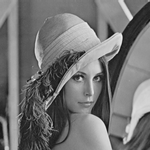
\includegraphics[width=0.2\textwidth]{lenaGray}\\
   \caption{$125\times 125$ Grayscale Lena}
\end{figure}
\subsection{Σύνθεση}

Το επόμενο βήμα μετά την επιτυχή προσομοίωση της συνάρτησής μας είναι η σύνθεσή της. Αν όλα είναι σωστά, παράγεται κώδικας VHDL ή Verilog καθώς επίσης μία αναφορά όπου φαίνεται η αξιοποίηση των πόρων και οι χρονισμοί όλων των instances του προγράμματος μας. Σε αντίθετη περίπτωση, το πρόγραμμα εμφανίζει τα σφάλματα και τις παρατηρήσεις ώστε αυτές να διορθωθούν και να επαναληφθεί η διαδικασία της σύνθεσης.

Σε αυτό το σημείο μπορούν να δημιουργηθούν νέα solutions (δεν είναι αναγκαίο) και να εφαρμοστούν βελτιστοποιήσεις που θα βελτιώσουν την απόδοση του υλικού που σχεδιάστηκε.

\subsection{RTL Co-Simulation}

Μετά την επιτυχή βελτίωση του προγράμματος μας και την επίτευξη των προδιαγραφών που έχουμε ορίσει πραγματοποιούμε την προσομοίωση σε επίπεδο RTL. Σε αυτό το στάδιο προσομοιώνεται ο κώδικας με τη βοήθεια του testbench με τη διαφορά ότι σε αυτό το στάδιο ελέγχεται το hardware (VHDL, Verilog, SystemC) που παράχθηκε στο προηγούμενο βήμα. Υπάρχει υποστήριξη για 3rd party προσομοιωτές όπως τα XSim, ISim.
\begin{figure}[H]
   \centering
   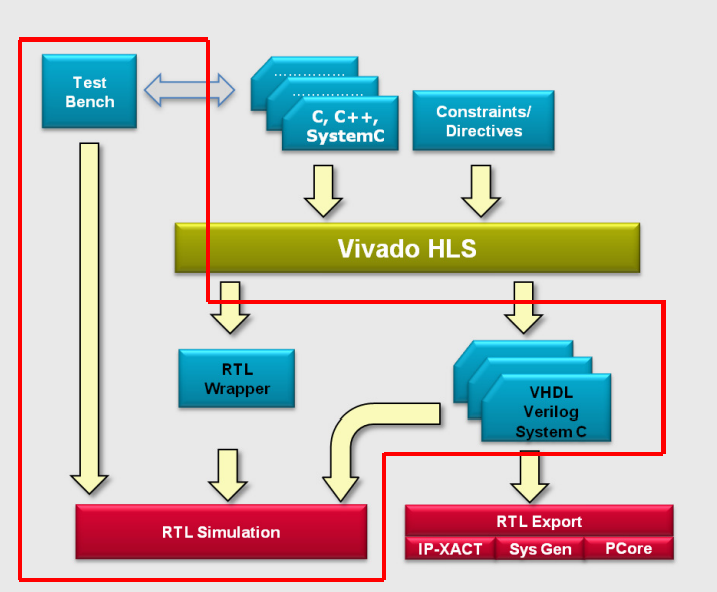
\includegraphics[width=0.8\textwidth]{hlsappflow}\\
   \caption{Ροή RTL CO-SIM \cite{ug902}}
\end{figure}

Τα αποτελέσματα της προσομοίωσης εμφανίζονται στην κονσόλα και παράγεται επίσης μία αναφορά που μας ενημερώνει για την επιτυχία/αποτυχία της προσομοίωσης καθώς και για τους κύκλους ρολογιού που απαιτεί το πρόγραμμα μας.
\begin{table}[H]
\centering
\caption{Αναφορά Co-Sim}
\label{my-label}
\begin{tabular}{@{}rcccclll@{}}
\toprule
\multicolumn{1}{l}{} & \multicolumn{4}{c}{Latency} & \multicolumn{3}{c}{Interval} \\ \midrule
RTL & Status & min & avg & max & min & avg & max \\
VHDL & N/A & N/A  & N/A  & N/A  & N/A & N/A & N/A \\
Verilog & 93304  & 93304  & 93304  & N/A & N/A & N/A & N/A \\ \bottomrule
\end{tabular}
\end{table}

\subsection{IP Export}

Τελικό βήμα στη ροή σχεδιασμού HLS είναι η εξαγωγή του υλικού για την χρήση του. Οι διαθέσιμοι τύποι είναι οι ακόλουθοι:
\begin{itemize}[leftmargin=*]
	\item{IP-XACT για τη χρήση στο Vivado - Σειρά 7 \& Zynq μόνο}
	\item{System Generator IP block - Σειρά 7 \& Zynq μόνο}
	\item{Pcore IP block για χρήση σε EDK - Σειρά 7, Zynq, Spartan-3, Spartan-6, Virtex-4/5/6} \\
\end{itemize}

Επιλέχθηκε η πρώτη περίπτωση - IP-XACT καθώς διευκολύνει κατά μεγάλο βαθμό τη διαδικασία δημιουργίας του πλήρους συστήματος στο Vivado που θα αναλυθεί στη συνέχεια.
\subsection{TCL}

Η γλώσσα TCL - Tool Command Language είναι μία γλώσσα προγραμματισμού ενσωματωμένη στη πλατφόρμα Vivado. Αποτελεί μία από τις πρότυπες γλώσσες στη βιομηχανία των ημιαγωγών σε εφαρμογές προγραμματισμού διεπαφών.

Η TCL επιτρέπει την εκτέλεση αυτοματοποιημένων scripts σε όλα τα στάδια της σχεδιαστικής ροής στην πλατφόρμα Vivado, γεγονός που την καθιστά υπερβολικά χρήσιμη. Η μεταφορά του προγράμματος σε κάποιο άλλο υπολογιστικό σύστημα, η εκτέλεση της σύνθεσης, η προσομοίωση και η εξαγωγή μπορούν να πραγματοποιηθούν χωρίς την εκτέλεση των προγραμμάτων σε γραφικών περιβάλλον αλλά από το terminal/cmd, εξοικονομώντας έτσι πολύτιμο χρόνο.

To HLS παράγει από μόνο του δύο αρχεία TCL: \textbf{script.tcl} και \textbf{directives.tcl}. Το πρώτο αρχείο είναι υπεύθυνο για τη προσομοίωση, τη σύνθεση και την εξαγωγή του υλκού ενώ στο δεύτερο είναι αποθηκευμένα τα διάφορα \textbf{\#pragmas} για τη βελτιστοποίηση της σύνθεσης.

Με τη βοήθεια του command prompt του Vivado και την εντολή \textbf{vivado\textunderscore hls -f script.tcl} μπορούμε να εκτελέσουμε όλες τις παραπάνω λειτουργίες χωρίς τη χρήση κάποιου GUI.
\section{Vivado IP Integrator} \label{Vivado}

Το Vivado IP Integrator επιτρέπει στο σχεδιαστή να δημιουργεί πολύπλοκα σχέδια συστημάτων διασυνδέοντας IP μέσω του IP καταλόγου της Xilinx και του ίδιου του σχεδιαστή. Τα σχέδια μπορούν να σχεδιαστούν διαδραστικά μέσω του γραφικού περιβάλλοντος αλλά και μέσω TCL αρχείων. Το Vivado IPI δίνει τη δυνατότητα κατασκευής του σχεδιασμού στο επίπεδο διεπαφής καθώς και στο επίπεδο πυλών όπου χρειάζεται περισσότερη ακρίβεια.

Μια διεπαφή, όπως για παράδειγμα το AXI4-Stream, περιέχει έναν μεγάλο αριθμό σημάτων και διασυνδέσεων. Αν κάθε σήμα ή διασύνδεση ήταν ορατά σε ένα IP block, τότε το συνολικό block design θα ήταν υπερβολικά περίπλοκο. Τo Vivado ομαδοποιεί αυτά τα σήματα και διασυνδέσεις ώστε να αντιμετωπιστεί αυτό το πρόβλημα. Στο ακόλουθο σχήμα φαίνεται μία απλοποιημένη ροή σχεδιασμού στο Vivado.
\begin{figure}[H]
\begin{center}
\begin{tikzpicture}[
    node distance = 5mm and 8mm,
    start chain = going below,
  	alg/.style = {draw, align=center, font=\linespread{0.8}\selectfont}]
    \begin{scope}[every node/.append style={on chain, join=by -Stealth}]
		\node (n1) [alg]  {Block design \\ creation};
		\node (n2) [alg]  {IP blocks \\ import};
		\node (n3) [alg]  {Customizing \& \\ connecting};
		\node (n4) [alg]  {Design \\ Validation};
		\node (n5) [alg]  {Generating \\ Output Products};
		\node (n6) [alg]  {HDL Wrapper \\ Creation};
		\node (n7) [alg]  {Implementation \& \\ Synthesis};
		\node (n8) [alg]  {Bitstream \\ Generation};
		\node (n9) [alg]  {HW export \& \\ SDK launch};
    \end{scope}
    \end{tikzpicture}
\end{center}
\caption{Βασική ροή σχεδιασμού στο Vivado IPI}
\end{figure}
\subsection{Δημιουργία Project}

Στην αρχική οθόνη του Vivado, επιλέγουμε τη δημιουργία νέου project. Στο παράθυρο που εμφανίζεται:
\begin{enumerate}[label=(\alph*)]
\item {Διαλέγουμε ένα όνομα και στη συνέχεια πατάμε στο \textbf{Next}}
\item {Σαν τοποθεσία αποθήκευσης του project επιλέγουμε το φάκελο που περιέχει το HLS project}
\item {Επιλέγουμε το \textbf{Do not specify sources at this time}}
\item {Πατάμε \textbf{Next}} \\
\end{enumerate}
Στη σελίδα Default Part:
\begin{enumerate}[label=(\alph*)]
\item {Πατάμε στο \textbf{Boards}}
\item {Επιλέγουμε το \textbf{ZYNQ-7 ZC702 Evaluation Board}}
\item {Πατάμε \textbf{Next} και στη συνέχεια \textbf{Finish}}
\end{enumerate}

\subsection{Δημιουργία Σχεδίου \& Εισαγωγή IP}

Σκοπός αυτού του βήματος είναι η εισαγωγή του IP block που σχεδιάσαμε με τη βοήθεια του Vivado HLS και η δημιουργία ενός block design όπου θα πραγματοποιηθεί η διασύνδεση όλων των απαραίτητων block του συνολικού συστήματος. Στις ρυθμίσεις του project επιλέγουμε το φάκελο που περιέχει το IP block - στη περίπτωση μας ονομάζεται \textbf{canny}.

Στη συνέχεια δημιουργούμε ένα νέο block design και του δίνουμε το επιθυμητό όνομα. Σε αυτό το σημείο πρέπει να καθοριστεί ποια είναι τα περιφερειακά που χρειάζονται για το σύστημά μας με βάση τις προδιαγραφές που έχουμε ορίσει. Τα βασικά περιφερειακά που απαιτούνται είναι τα εξής:
\begin{itemize}
	\item{ZYNQ7 Processing System}
	\item{Canny IP}
	\item{AXI Direct Memory Access} \\
\end{itemize}

\begin{figure}[H]
   \centering
   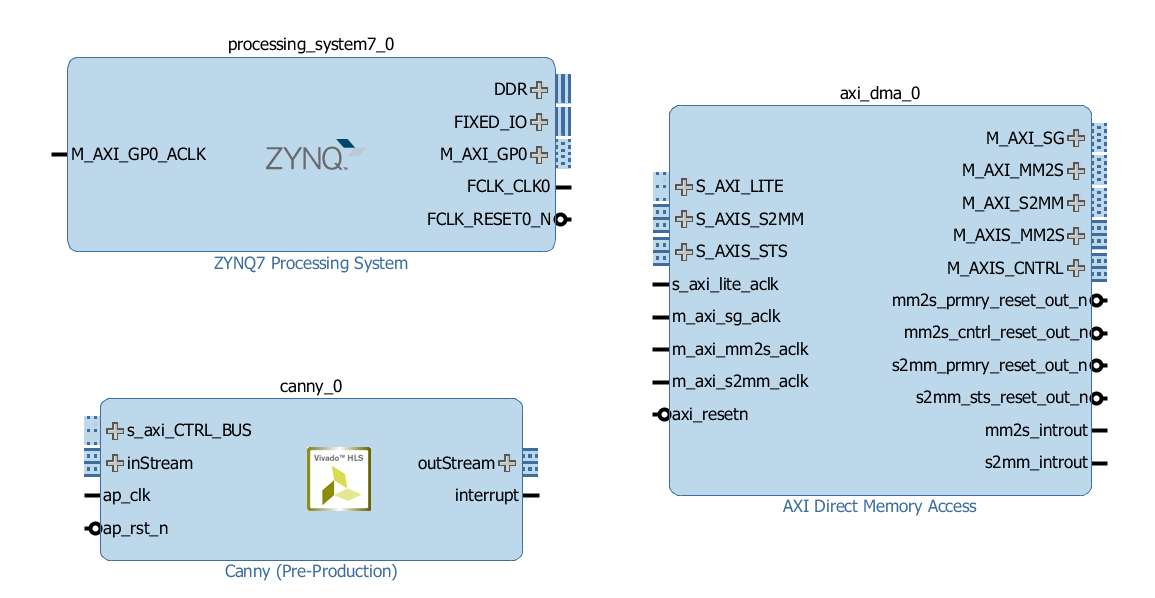
\includegraphics[width=0.8\textwidth]{vivadoblocks}\\
   \caption{Βασικά IP Block}
\end{figure}

\subsection{Παραμετροποίηση, Διασύνδεση \& Επαλήθευση}

Το Vivado έχει τη δυνατότητα να πραγματοποιήσει αυτόματα τις διασυνδέσεις των περιφερειακών και των διάφορων διεπαφών του συστήματος, απλοποιώντας σημαντικά τη διαδικασία. Αρχικά, εισάγουμε το \textbf{ZYNQ7 Processing System} και πραγματοποιούμε τις ακόλουθες ρυθμίσεις:
\begin{itemize}
	\item{Εφαρμογή ZC702 Preset}
	\item{Ενεργοποίηση των PL-PS Interrupts - IRQ\textunderscore F2P[15:0]}
	\item{Ρύθμιση του ρολογιού του FPGA ίσο με 100 MHz}
	\item{Ενεργοποίηση των διεπαφών S AXI HP0 και M AXI GP0}\\
\end{itemize}

Επιλέγουμε την εντολή \textbf{Run Block Automation} η οποία ρυθμίζει το ZYNQ7 PS. Στη συνέχεια εισάγουμε το IP μας και επιλέγουμε την εντολή \textbf{Run Connection Automation} η οποία το διασυνδέει με το περιφερειακό μας.

Παρατηρούμε ότι το Vivado εισήγαγε τα Processor System Reset και AXI Interconnect IPs, τα οποία είναι υπεύθυνα για τα reset σήματα και τις διασυνδέσεις AXI αντίστοιχα. Έκανε επίσης όλες τις απαραίτητες συνδέσεις και ρυθμίσεις.
\begin{figure}[H]
   \centering
   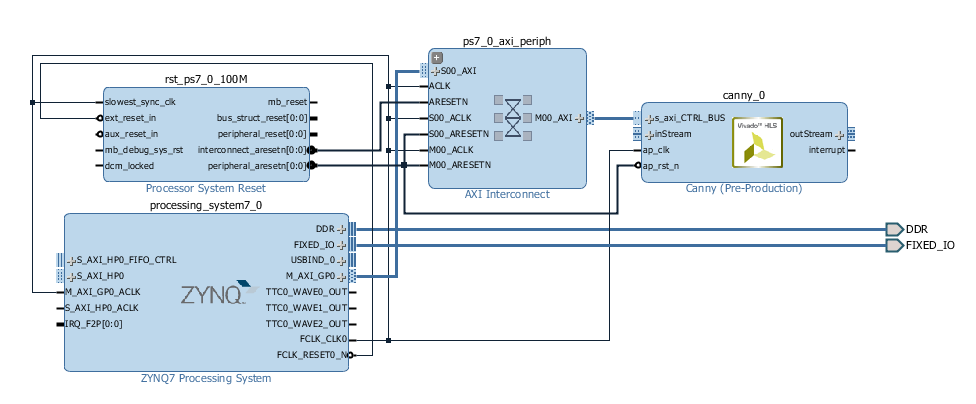
\includegraphics[width=\textwidth]{vivadoBlockAuto}\\
   \caption{Διασύνδεση βασικών IP Blocks}
\end{figure}

Σειρά έχει η εισαγωγή του AXI DMA περιφερειακού. Με αντίστοιχο τρόπο το εισάγουμε στο design μας και κάνουμε τις απαραίτητες αλλαγές. Ρυθμίζουμε το DMA όπως φαίνεται στην εικόνα, ενεργοποιώντας τον απλό τρόπο λειτουργίας και όχι τον τρόπο \textbf{Scatter-Gather}.

Στον απλό τρόπο λειτουργίας οι μεταφορές δεδομένων θα πρέπει να ελεγθούν μέσω της εφαρμογής που θα αναπτυχθεί στο SDK. Περιλαμβάνει δύο κανάλια: ένα από το DMA προς τη συσκευή και ένα από τη συσκευή προς το DMA. Η εφαρμογή που θα αναπτυχθεί πρέπει να ορίσει τη διεύθυνση του buffer καθώς και το μέγεθος του ώστε να ξεκινήσει η μεταφορά δεδομένων στο αντίστοιχο κανάλι. Αντίθετα, στο Scatter-Gather τρόπο λειτουργίας, η εφαρμογή ορίζει μία λίστα ανταλλαγών δεδομένων τις οποίες επεξεργάζεται το υλικό χωρίς περαιτέρω παρεμβολή του επεξεργαστή. Κατά τη διάρκεια της μεταφοράς, η εφαρμογή μπορεί να προσθέτει επιπλέον εργασίες στο υλικό.

Στη συνέχεια πραγματοποιούνται όλες οι συνδέσεις μεταξύ όλων των περιφερειακών και του ZYNQ7. Το Vivado όμως παρέλειψε τις συνδέσεις των interrupts, και των εισόδων και εξόδων δεδομένων του AXI4-Stream από και προς το DMA, οι οποίες πρέπει να γίνουν χειροκίνητα. Ενώνουμε επομένως το inStream του Canny με το \textbf{M\_AXIS\_MM2S} και το outStream με το \textbf{S\_AXIS\_S2MM}. Καθώς ο αριθμός των απαιτούμενων σημάτων διακοπών είναι τρείς, θα προσθέσουμε ένα \textbf{concat block} το οποίο θα συνενώσει τα interrupts του DMA και του Canny και θα συνδεθεί με το interrupt port του ZYNQ7. Σε περίπτωση που αποφασίσουμε να χρησιμοποιήσουμε τον ελεγκτή DMA με polling, το παραπάνω βήμα μπορεί να παραλειφθεί και το interrupt του Canny συνδέεται απευθείας στο \textbf{ZYNQ7}. Τέλος, ελέγχουμε αν έχουν οριστεί διευθύνσεις για τα περιφερειακά.
\begin{figure}[H]
   \centering
   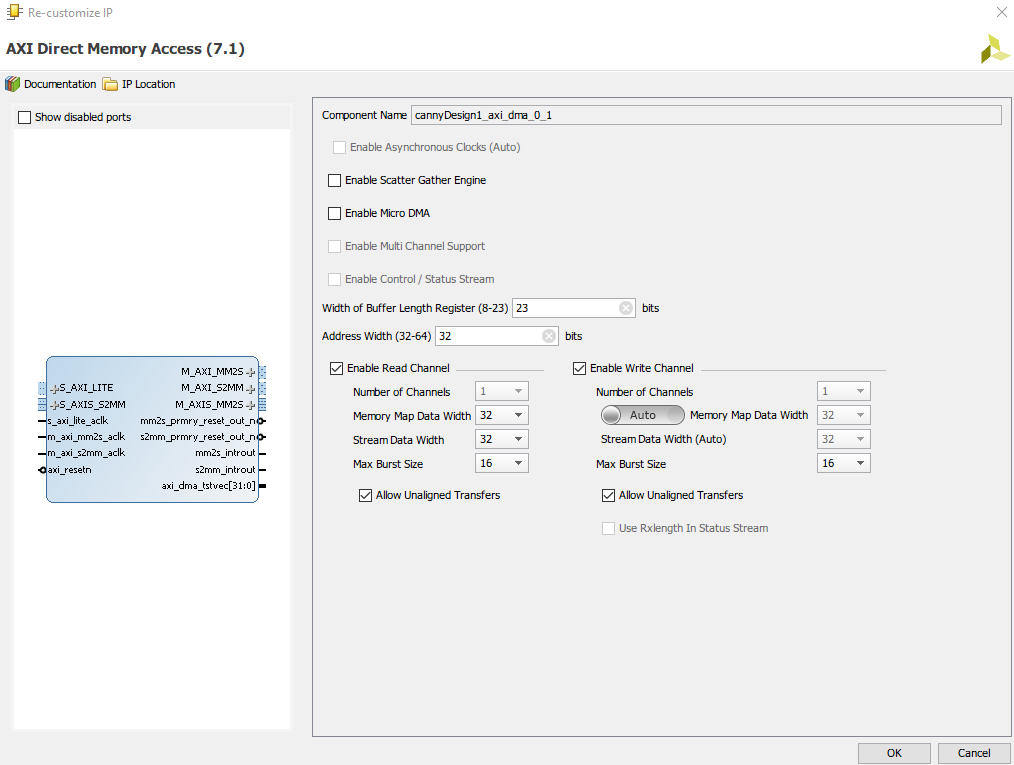
\includegraphics[width=0.8\textwidth]{dma}\\
   \caption{Ρύθμιση AXI Direct Memory Access}
\end{figure}
\subsection{Σύνθεση, bitstream \& εξαγωγή στο SDK}

\begin{itemize}[label={},leftmargin=*]
\item \textbf{Output products generation}

Η εντολή αυτή παραθέτει όλα τους IP πυρήνες του σχεδίου μας και παράγει τα απαιτούμενα αποτελέσματα, όπως για παράδειγμα, πρότυπα των instances, HDL, περιορισμούς, αρχεία προσομοίωσης κά. \\
\item \textbf{HDL Wrapper Creation}

Με την εντολή αυτή ορίζεται ένα HDL wrapper για τον τρέχοντα σχεδιασμό που το ορίζει ως το top-level σχεδιασμό, επιτρέποντας τη σύνθεση, υλοποίηση και την παραγωγή του bitstream. \\
\end{itemize}

Αφου βεβαιώσουμε ότι έχουν πραγματοποιηθεί όλες οι απαραίτητες συνδέσεις επιλέγουμε \textbf{Validate Design} ώστε να ελεγχθεί το σύστημα μας. Στη συνέχεια από το παράθυρο \textbf{Sources} επιλέγουμε το \textbf{Generate output products} και στη συνέχεια \textbf{Generate HDL Wrapper}. Επόμενο βήμα είναι η εκτέλεση της υλοποίησης.
\begin{figure}[H]
   \centering
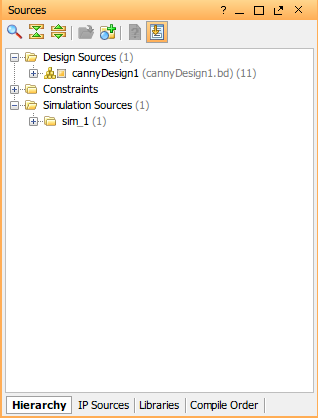
\includegraphics[width=0.45\textwidth]{sources}
   \caption{Sources window}
\end{figure}

Τελευταίο βήμα είναι η σύνθεση, η υλοποίηση και η παραγωγή του αρχείο προγραμματισμού του FPGA. Με την εντολή \textbf{Generate Bitstream} πραγματοποιούνται αυτές οι εργασίες. Το Vivado δημιουργεί μία αναφορά για τους απαραίτητους πόρους, τις εκτιμήσεις κατανάλωσης κά. Δημιουργείται επίσης και μία άποψη του FPGA Fabric με όλα τα κατασκευαστικά blocks που χρειάστηκαν για την υλοποίηση του πλήρους συστήματος.

Επιλέγοντας \textbf{Export Hardware}, εξάγουμε το υλικό ώστε να το χρησιμοποιήσουμε για τον προγραμματισμό του μέσω του SDK, το οποίο εκτελείται μέσω την εντολής \textbf{Launch SDK}.
\newpage
\begin{figure}[H]
   \centering
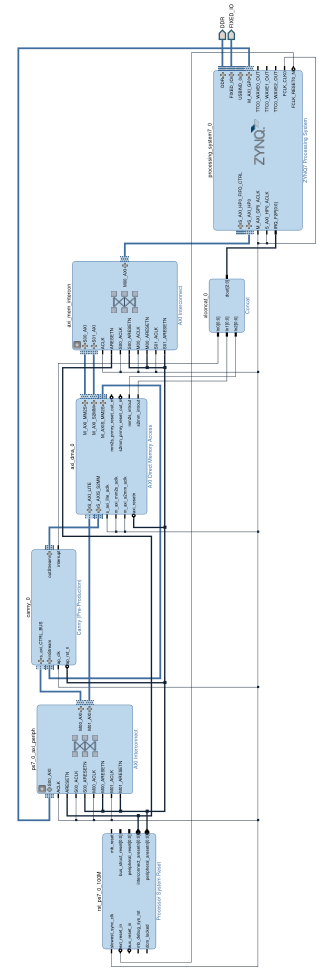
\includegraphics[height=22cm]{fullPNG}
   \caption{Πλήρες σύστημα}
\end{figure}
\newpage
\section{SDK}\label{SDK}

Σκοπός του Software Development Kit (SDK) της Xilinx είναι ο έλεγχος του επεξεργαστικού συστήματος που αποτελείται από 2 ARM πυρήνες. Το Vivado κατά την εξαγωγή του υλικού δημιουργεί μία πλατφόρμα που περιέχει το σύστημα που σχεδιάστηκε και στην οποία βασιζόμαστε για να αναπτύξουμε τον κώδικα μας.

Το πρώτο βήμα είναι η δημιουργία ενός νέου application project όπου επιλέγουμε το όνομα του, την πλατφόρμα στην οποία θα βασιστεί το project μας. Στο επόμενο βήμα, είναι σκόπιμο να επιλεχθεί η έτοιμη εφαρμογή `hello world' καθώς περιέχει header αρχεία τα οποία είναι απαραίτητα για τη σωστή λειτουργία του προγράμματος μας και δεν περιέχονται έαν είχαμε επιλέξει μία κενή εφαρμογή.

Σκοπός μας είναι η ανάπτυξη μίας εφαρμογής η οποία θα αρχικοποιεί τον DMA ελεγκτή και τις διακοπές ώστε να πραγματοποιείται μεταφορά δεδομένων ανάμεσα στο FPGA και στον επεξεργαστή και θα καλεί τον αλγορίθμο που αναπτύχθηκε στο HLS. Τέλος, θα πραγματοποιείται η έξοδος των δεδομένων μέσω της διεπαφής UART προς τον ΗΥ όπου θα αποθηκεύεται η εικόνα ώστε να έχουμε και μία οπτική απεικόνιση των αποτελεσμάτων. Η βασική ροή της εφαρμογής είναι η εξής:
\begin{figure}[H]
\begin{center}
\begin{tikzpicture}[
    node distance = 4mm and 6mm,
    start chain = going right,
  	alg/.style = {draw, align=center, font=\linespread{0.8}\selectfont}]
    \begin{scope}[every node/.append style={on chain, join=by -Stealth}]
		\node (n1) [alg]  {DMA, Canny \\ Instances};
		\node (n2) [alg]  {Αρχικοποίηση \\ IP};
		\node (n3) [alg]  {Εκκίνηση \\ IP};
		% \node (n4) [alg]  {Μεταφορά \\ δεδομένων};
		\node (n5) [alg]  {Λήψη \\ δεδομένων};
    \end{scope}
    \end{tikzpicture}
\end{center}
\caption{Ροή εφαρμογής ARM}
\end{figure}
\subsection{Απαραίτητα αρχεία}

Τα βασικά αρχεία που θα χρησιμοποιηθούν και πρέπει να συμπεριληφθούν στον κώδικά μας είναι τα \textbf{xcanny.c} και \textbf{xparameters.h}. Το πρώτο αρχείο, αποτελεί τους drivers του IP Block μας και δημιουργήθηκε από το Vivado HLS κατά τη διαδικασία εξαγωγής σε IP. Περιλαμβάνει τις διάφορες εντολές για την εκκίνηση της λειτουργίας, τον έλεγχο της κατάστασής του (idle, ready, done) καθώς και εντολές για το χειρισμό των αιτήσεων διακοπών. Το δεύτερο αρχείο δημιουργήθηκε από το Vivado και περιέχει τις απαιτούμενες τιμές των περιφερειακών όπως για παράδειγμα τις διευθύνσεις των διεπαφών του AXI4, τις διευθύνσεις της DDR μνήμης κά.

Δύο εξίσου σημαντικά αρχεία είναι τα \textbf{xaxidma.h} και \textbf{xscugic.h}. Το πρώτο περιλαμβάνει τις απαραίτητες συναρτήσεις για την αρχικοποίηση και τον έλεγχο του DMA ελεγκτή ενώ το δεύτερο είναι ο ελεγκτής των αιτήσεων διακοπών. Περιλαμβάνει όλες τις δομές και συναρτήσεις για τον πλήρη έλεγχο των διακοπών του υπολογιστικού συστήματος. Τέλος, τα δεδομένα εισόδου της εικόνας σε grayscale μορφή είναι αποθηκευμένα σε ένα header αρχείο.

\begin{lstlisting}[language=C++,belowskip=-0.3\baselineskip]
	#include <stdio.h>
	#include "stdlib.h"
	#include "platform.h"
	#include "xcanny.h"
	#include "xparameters.h"
	#include "xaxidma.h"
	#include "xscugic.h"
\end{lstlisting}

\subsection{Δομή κώδικα}

Αρχικά, σε αντίθεση με τη ροή σχεδιασμού στο HLS, η κύρια συνάρτηση είναι η \textbf{main( )}. Έχει οριστεί επίσης μία συνάρτηση, η \textbf{initPeripherals( )}.

Δημιουργείται ένα instance για τους drivers του ελεγκτή DMA που θα χρησιμοποιηθεί και στη συνέχεια ορίζεται η δομή των ρυθμίσεων διαμόρφωσης για τους drivers που δημιουργήθηκαν προηγουμένως. Αντίστοιχα, πραγματοποιούνται οι ίδιες λειτουργίες για το canny IP Block. Η λειτουργία των δομών αυτών είναι η μεταφορά πληροφοριών του υλικού από την εφαρμογή στους drivers.
\begin{lstlisting}[language=C++,belowskip=-0.3\baselineskip]
//DMA Instance
XAxiDma 		AxiDma;
XAxiDma_Config	*AxiDma_cfg;
//Canny IP Instance
XCanny			xCanny;
XCanny_Config	*xCanny_cfg;
\end{lstlisting}
\begin{itemize}[label={},leftmargin=*]

\item \textbf{main( )}

Ο σκοπός της κύριας συνάρτησης είναι η εκκίνηση του Canny IP με σκοπό τη λήψη δεδομένων αφότου πραγματοποιηθεί η επεξεργασία τους στο FPGA fabric. Γίνονται συνεχείς έλεγχοι για τη σωστή λειτουργία της μεταφοράς δεδομένων. Ζητείται επίσης, από το χρήστη να εισάγει μία τιμή κατωφλίωσης. Η εισαγωγή της τιμής σηματοδοτεί επίσης την έναρξη της επεξεργασίας των δεδομένων της εικόνας. Αφότου ολοκληρωθεί η λήψη των επεξεργασμένων δεδομένων, αυτά αποστέλλονται μέσω της διεπαφής UART στον ΗΥ όπου τα λαμβάνουμε με τη βοήθεια του PuTTY και τα αποθηκεύουμε σε αρχείο εικόνας ώστε να αξιολογηθούν.

Για να πραγματοποιηθεί μία απλή μεταφορά δεδομένων τόσο από τον επεξεργαστή προς το περιφερειακό όσο και από το περιφερειακό προς τον επεξεργαστή χρησιμοποιείται η εντολή \textbf{XAxiDma\_SimpleTransfer(XAxiDma *InstancePtr, UINTPTR BuffAddr, u32 Length,	int Direction)}. Το τμήμα κώδικα που εκτελεί τις συγκεκριμένες λειτουργίες είναι το εξής:

\begin{lstlisting}[language=C++,belowskip=-0.3\baselineskip]
// Receiving output data from Canny IP
status = 	XAxiDma_SimpleTransfer(&AxiDma, (u32)outBuffer, ARRAY_SIZE*sizeof(int), XAXIDMA_DEVICE_TO_DMA);
if (status != XST_SUCCESS) {
	printf("Error: DMA transfer from Vivado HLS block failed\n");
	return XST_FAILURE;
}
while (XAxiDma_Busy(&AxiDma, XAXIDMA_DEVICE_TO_DMA)) ;
printf("Success: Received results!\r\n");
\end{lstlisting}

Για τον έλεγχο της κατάστασης του περιφερειακού μας μπορούμε να χρησιμοποιήσουμε τις εντολές που μας παρέχονται από τους drivers που παρήχθησαν μέσω της διαδικασίας εξαγωγής του IP μας. Αυτές είναι οι \textbf{isDone}, \textbf{isIdle}, \textbf{isReady}. \\
\begin{lstlisting}[language=C++,belowskip=-0.3\baselineskip]
int isDone, isIdle, isReady;

isDone = XCanny_IsDone(&xCanny);
isIdle = XCanny_IsIdle(&xCanny);
isReady = XCanny_IsReady(&xCanny);
printf("Canny edge detector: isDone %d, isIdle %d, isReady%d\r\n", isDone, isIdle, isReady);
\end{lstlisting}

Aφότου πραγματοποιηθεί η λήψη των δεδομένων και πριν τη χρήση τους, πρέπει να πραγματοποιήσουμε το "invalidation" τους ώστε η προσπέλασή τους να είναι επιτυχής. Οι διαδικασίες αυτές πραγματοποιούνται ως εξής:
\begin{lstlisting}[language=C++,belowskip=-0.3\baselineskip]
Xil_DCacheFlushRange((int)output,ARRAY_SIZE*sizeof(int));

// Perform receive function

Xil_DCacheInvalidateRange((u32)outBuffer, ARRAY_SIZE*sizeof(int));

// Use data
\end{lstlisting}

\item \textbf{initPeripherals( )}

Βασικός σκοπός της συγκεκριμένης συνάρτησης είναι η αρχικοποίηση των API κλήσεων των drivers του DMA και του Canny και εκκίνηση των περιφερειακών του συστήματος. Παράλληλα, πραγματοποιούνται έλεγχοι ώστε να επιβεβαιωθεί ότι τα περιφερειακά έχουν αρχικοποιηθεί σωστά και είναι λειτουργικά. Στην περίπτωση που υπάρχει κάποιο πρόβλημα, η εκτέλεση του προγράμματος τερματίζεται αυτόματα.
\begin{lstlisting}[language=C++,belowskip=-0.3\baselineskip]
int status ;
// Init Canny Core
printf("\nInitialization of Canny IP Block\n");
xCanny_cfg = XCanny_LookupConfig(XPAR_CANNY_0_DEVICE_ID);
if (xCanny_cfg) {
	int status = XCanny_CfgInitialize(&xCanny, xCanny_cfg);
	if (status != XST_SUCCESS)
		printf("Error initializing Canny IP\n");
	else
		printf("\r\nSuccessfully initialized Canny IP\n");
}

// Init axiDMA Core
printf("\nInitialization of AXI DMA Core\n");
AxiDma_cfg = XAxiDma_LookupConfig(XPAR_AXIDMA_0_DEVICE_ID);
if (AxiDma_cfg) {
	int status = XAxiDma_CfgInitialize(&AxiDma, AxiDma_cfg);
	if (status != XST_SUCCESS)
		printf("Error initializing AXI DMA Core\n");
	else
		printf("Success AXIDMA\n");
}
\end{lstlisting}

\end{itemize}

